% Options for packages loaded elsewhere
% Options for packages loaded elsewhere
\PassOptionsToPackage{unicode}{hyperref}
\PassOptionsToPackage{hyphens}{url}
\PassOptionsToPackage{dvipsnames,svgnames,x11names}{xcolor}
%
\documentclass[
  11pt,
  letterpaper,
  DIV=11,
  numbers=noendperiod]{scrartcl}
\usepackage{xcolor}
\usepackage[margin=2.5cm]{geometry}
\usepackage{amsmath,amssymb}
\setcounter{secnumdepth}{5}
\usepackage{iftex}
\ifPDFTeX
  \usepackage[T1]{fontenc}
  \usepackage[utf8]{inputenc}
  \usepackage{textcomp} % provide euro and other symbols
\else % if luatex or xetex
  \usepackage{unicode-math} % this also loads fontspec
  \defaultfontfeatures{Scale=MatchLowercase}
  \defaultfontfeatures[\rmfamily]{Ligatures=TeX,Scale=1}
\fi
\usepackage{lmodern}
\ifPDFTeX\else
  % xetex/luatex font selection
  \setmainfont[]{Palatino Linotype}
  \setmonofont[]{Consolas}
\fi
% Use upquote if available, for straight quotes in verbatim environments
\IfFileExists{upquote.sty}{\usepackage{upquote}}{}
\IfFileExists{microtype.sty}{% use microtype if available
  \usepackage[]{microtype}
  \UseMicrotypeSet[protrusion]{basicmath} % disable protrusion for tt fonts
}{}
\usepackage{setspace}
\makeatletter
\@ifundefined{KOMAClassName}{% if non-KOMA class
  \IfFileExists{parskip.sty}{%
    \usepackage{parskip}
  }{% else
    \setlength{\parindent}{0pt}
    \setlength{\parskip}{6pt plus 2pt minus 1pt}}
}{% if KOMA class
  \KOMAoptions{parskip=half}}
\makeatother
% Make \paragraph and \subparagraph free-standing
\makeatletter
\ifx\paragraph\undefined\else
  \let\oldparagraph\paragraph
  \renewcommand{\paragraph}{
    \@ifstar
      \xxxParagraphStar
      \xxxParagraphNoStar
  }
  \newcommand{\xxxParagraphStar}[1]{\oldparagraph*{#1}\mbox{}}
  \newcommand{\xxxParagraphNoStar}[1]{\oldparagraph{#1}\mbox{}}
\fi
\ifx\subparagraph\undefined\else
  \let\oldsubparagraph\subparagraph
  \renewcommand{\subparagraph}{
    \@ifstar
      \xxxSubParagraphStar
      \xxxSubParagraphNoStar
  }
  \newcommand{\xxxSubParagraphStar}[1]{\oldsubparagraph*{#1}\mbox{}}
  \newcommand{\xxxSubParagraphNoStar}[1]{\oldsubparagraph{#1}\mbox{}}
\fi
\makeatother

\usepackage{color}
\usepackage{fancyvrb}
\newcommand{\VerbBar}{|}
\newcommand{\VERB}{\Verb[commandchars=\\\{\}]}
\DefineVerbatimEnvironment{Highlighting}{Verbatim}{commandchars=\\\{\}}
% Add ',fontsize=\small' for more characters per line
\usepackage{framed}
\definecolor{shadecolor}{RGB}{241,243,245}
\newenvironment{Shaded}{\begin{snugshade}}{\end{snugshade}}
\newcommand{\AlertTok}[1]{\textcolor[rgb]{0.68,0.00,0.00}{#1}}
\newcommand{\AnnotationTok}[1]{\textcolor[rgb]{0.37,0.37,0.37}{#1}}
\newcommand{\AttributeTok}[1]{\textcolor[rgb]{0.40,0.45,0.13}{#1}}
\newcommand{\BaseNTok}[1]{\textcolor[rgb]{0.68,0.00,0.00}{#1}}
\newcommand{\BuiltInTok}[1]{\textcolor[rgb]{0.00,0.23,0.31}{#1}}
\newcommand{\CharTok}[1]{\textcolor[rgb]{0.13,0.47,0.30}{#1}}
\newcommand{\CommentTok}[1]{\textcolor[rgb]{0.37,0.37,0.37}{#1}}
\newcommand{\CommentVarTok}[1]{\textcolor[rgb]{0.37,0.37,0.37}{\textit{#1}}}
\newcommand{\ConstantTok}[1]{\textcolor[rgb]{0.56,0.35,0.01}{#1}}
\newcommand{\ControlFlowTok}[1]{\textcolor[rgb]{0.00,0.23,0.31}{\textbf{#1}}}
\newcommand{\DataTypeTok}[1]{\textcolor[rgb]{0.68,0.00,0.00}{#1}}
\newcommand{\DecValTok}[1]{\textcolor[rgb]{0.68,0.00,0.00}{#1}}
\newcommand{\DocumentationTok}[1]{\textcolor[rgb]{0.37,0.37,0.37}{\textit{#1}}}
\newcommand{\ErrorTok}[1]{\textcolor[rgb]{0.68,0.00,0.00}{#1}}
\newcommand{\ExtensionTok}[1]{\textcolor[rgb]{0.00,0.23,0.31}{#1}}
\newcommand{\FloatTok}[1]{\textcolor[rgb]{0.68,0.00,0.00}{#1}}
\newcommand{\FunctionTok}[1]{\textcolor[rgb]{0.28,0.35,0.67}{#1}}
\newcommand{\ImportTok}[1]{\textcolor[rgb]{0.00,0.46,0.62}{#1}}
\newcommand{\InformationTok}[1]{\textcolor[rgb]{0.37,0.37,0.37}{#1}}
\newcommand{\KeywordTok}[1]{\textcolor[rgb]{0.00,0.23,0.31}{\textbf{#1}}}
\newcommand{\NormalTok}[1]{\textcolor[rgb]{0.00,0.23,0.31}{#1}}
\newcommand{\OperatorTok}[1]{\textcolor[rgb]{0.37,0.37,0.37}{#1}}
\newcommand{\OtherTok}[1]{\textcolor[rgb]{0.00,0.23,0.31}{#1}}
\newcommand{\PreprocessorTok}[1]{\textcolor[rgb]{0.68,0.00,0.00}{#1}}
\newcommand{\RegionMarkerTok}[1]{\textcolor[rgb]{0.00,0.23,0.31}{#1}}
\newcommand{\SpecialCharTok}[1]{\textcolor[rgb]{0.37,0.37,0.37}{#1}}
\newcommand{\SpecialStringTok}[1]{\textcolor[rgb]{0.13,0.47,0.30}{#1}}
\newcommand{\StringTok}[1]{\textcolor[rgb]{0.13,0.47,0.30}{#1}}
\newcommand{\VariableTok}[1]{\textcolor[rgb]{0.07,0.07,0.07}{#1}}
\newcommand{\VerbatimStringTok}[1]{\textcolor[rgb]{0.13,0.47,0.30}{#1}}
\newcommand{\WarningTok}[1]{\textcolor[rgb]{0.37,0.37,0.37}{\textit{#1}}}

\usepackage{longtable,booktabs,array}
\usepackage{calc} % for calculating minipage widths
% Correct order of tables after \paragraph or \subparagraph
\usepackage{etoolbox}
\makeatletter
\patchcmd\longtable{\par}{\if@noskipsec\mbox{}\fi\par}{}{}
\makeatother
% Allow footnotes in longtable head/foot
\IfFileExists{footnotehyper.sty}{\usepackage{footnotehyper}}{\usepackage{footnote}}
\makesavenoteenv{longtable}
\usepackage{graphicx}
\makeatletter
\newsavebox\pandoc@box
\newcommand*\pandocbounded[1]{% scales image to fit in text height/width
  \sbox\pandoc@box{#1}%
  \Gscale@div\@tempa{\textheight}{\dimexpr\ht\pandoc@box+\dp\pandoc@box\relax}%
  \Gscale@div\@tempb{\linewidth}{\wd\pandoc@box}%
  \ifdim\@tempb\p@<\@tempa\p@\let\@tempa\@tempb\fi% select the smaller of both
  \ifdim\@tempa\p@<\p@\scalebox{\@tempa}{\usebox\pandoc@box}%
  \else\usebox{\pandoc@box}%
  \fi%
}
% Set default figure placement to htbp
\def\fps@figure{htbp}
\makeatother





\setlength{\emergencystretch}{3em} % prevent overfull lines

\providecommand{\tightlist}{%
  \setlength{\itemsep}{0pt}\setlength{\parskip}{0pt}}



 


\KOMAoption{captions}{tableheading}
\makeatletter
\@ifpackageloaded{caption}{}{\usepackage{caption}}
\AtBeginDocument{%
\ifdefined\contentsname
  \renewcommand*\contentsname{Table of contents}
\else
  \newcommand\contentsname{Table of contents}
\fi
\ifdefined\listfigurename
  \renewcommand*\listfigurename{List of Figures}
\else
  \newcommand\listfigurename{List of Figures}
\fi
\ifdefined\listtablename
  \renewcommand*\listtablename{List of Tables}
\else
  \newcommand\listtablename{List of Tables}
\fi
\ifdefined\figurename
  \renewcommand*\figurename{Figure}
\else
  \newcommand\figurename{Figure}
\fi
\ifdefined\tablename
  \renewcommand*\tablename{Table}
\else
  \newcommand\tablename{Table}
\fi
}
\@ifpackageloaded{float}{}{\usepackage{float}}
\floatstyle{ruled}
\@ifundefined{c@chapter}{\newfloat{codelisting}{h}{lop}}{\newfloat{codelisting}{h}{lop}[chapter]}
\floatname{codelisting}{Listing}
\newcommand*\listoflistings{\listof{codelisting}{List of Listings}}
\makeatother
\makeatletter
\makeatother
\makeatletter
\@ifpackageloaded{caption}{}{\usepackage{caption}}
\@ifpackageloaded{subcaption}{}{\usepackage{subcaption}}
\makeatother
\usepackage{bookmark}
\IfFileExists{xurl.sty}{\usepackage{xurl}}{} % add URL line breaks if available
\urlstyle{same}
\hypersetup{
  pdftitle={Global Supply Chain Pressure Index (GSCPI)},
  pdfauthor={Paolo Volterra},
  pdfkeywords={FED, indici, GSCPI, qmd},
  colorlinks=true,
  linkcolor={MidnightBlue},
  filecolor={Maroon},
  citecolor={Blue},
  urlcolor={Blue},
  pdfcreator={LaTeX via pandoc}}


\title{Global Supply Chain Pressure Index (GSCPI)}
\usepackage{etoolbox}
\makeatletter
\providecommand{\subtitle}[1]{% add subtitle to \maketitle
  \apptocmd{\@title}{\par {\large #1 \par}}{}{}
}
\makeatother
\subtitle{Studio sull'indicatore di stress della suppy chain elaborato
dalla Federal reserve}
\author{Paolo Volterra}
\date{}
\begin{document}
\maketitle

\renewcommand*\contentsname{Table of contents}
{
\hypersetup{linkcolor=}
\setcounter{tocdepth}{3}
\tableofcontents
}

\setstretch{1.5}
\begin{Shaded}
\begin{Highlighting}[]
\ImportTok{import}\NormalTok{ pandas }\ImportTok{as}\NormalTok{ pd}
\ImportTok{import}\NormalTok{ matplotlib.pyplot }\ImportTok{as}\NormalTok{ plt}
\ImportTok{import}\NormalTok{ requests}
\ImportTok{from}\NormalTok{ io }\ImportTok{import}\NormalTok{ BytesIO}

\CommentTok{\# 1. Scarica il file Excel dal sito ufficiale}
\NormalTok{url }\OperatorTok{=} \StringTok{"https://www.newyorkfed.org/medialibrary/research/interactives/gscpi/downloads/gscpi\_data.xlsx"}
\NormalTok{response }\OperatorTok{=}\NormalTok{ requests.get(url)}
\NormalTok{response.raise\_for\_status()}

\CommentTok{\# 2. Leggi la sheet \textquotesingle{}GSCPI Monthly Data\textquotesingle{} saltando le prime 5 righe}
\NormalTok{df }\OperatorTok{=}\NormalTok{ pd.read\_excel(}
\NormalTok{    BytesIO(response.content),}
\NormalTok{    sheet\_name}\OperatorTok{=}\StringTok{\textquotesingle{}GSCPI Monthly Data\textquotesingle{}}\NormalTok{,}
\NormalTok{    skiprows}\OperatorTok{=}\DecValTok{5}\NormalTok{,}
\NormalTok{    header}\OperatorTok{=}\VariableTok{None}\NormalTok{,}
\NormalTok{    usecols}\OperatorTok{=}\NormalTok{[}\DecValTok{0}\NormalTok{, }\DecValTok{1}\NormalTok{],  }\CommentTok{\# Solo colonne con data e GSCPI}
\NormalTok{    names}\OperatorTok{=}\NormalTok{[}\StringTok{\textquotesingle{}Date\textquotesingle{}}\NormalTok{, }\StringTok{\textquotesingle{}GSCPI\textquotesingle{}}\NormalTok{],}
\NormalTok{    decimal}\OperatorTok{=}\StringTok{\textquotesingle{},\textquotesingle{}}      \CommentTok{\# Usa la virgola come separatore decimale, se necessario}
\NormalTok{)}
\end{Highlighting}
\end{Shaded}

\begin{Shaded}
\begin{Highlighting}[]
\CommentTok{\# 3. Converti la colonna \textquotesingle{}Date\textquotesingle{} in datetime e imposta come indice}
\NormalTok{df[}\StringTok{\textquotesingle{}Date\textquotesingle{}}\NormalTok{] }\OperatorTok{=}\NormalTok{ pd.to\_datetime(df[}\StringTok{\textquotesingle{}Date\textquotesingle{}}\NormalTok{])}
\NormalTok{df.set\_index(}\StringTok{\textquotesingle{}Date\textquotesingle{}}\NormalTok{, inplace}\OperatorTok{=}\VariableTok{True}\NormalTok{)}

\CommentTok{\# 4. Plot}
\NormalTok{plt.figure(figsize}\OperatorTok{=}\NormalTok{(}\DecValTok{12}\NormalTok{, }\DecValTok{5}\NormalTok{))}
\NormalTok{plt.plot(df.index, df[}\StringTok{\textquotesingle{}GSCPI\textquotesingle{}}\NormalTok{], color}\OperatorTok{=}\StringTok{\textquotesingle{}darkblue\textquotesingle{}}\NormalTok{, linewidth}\OperatorTok{=}\DecValTok{2}\NormalTok{)}
\NormalTok{plt.axhline(}\DecValTok{0}\NormalTok{, linestyle}\OperatorTok{=}\StringTok{\textquotesingle{}{-}{-}\textquotesingle{}}\NormalTok{, color}\OperatorTok{=}\StringTok{\textquotesingle{}gray\textquotesingle{}}\NormalTok{)}
\NormalTok{plt.title(}\StringTok{\textquotesingle{}Global Supply Chain Pressure Index (GSCPI)\textquotesingle{}}\NormalTok{, fontsize}\OperatorTok{=}\DecValTok{15}\NormalTok{, fontweight}\OperatorTok{=}\StringTok{\textquotesingle{}bold\textquotesingle{}}\NormalTok{)}
\NormalTok{plt.xlabel(}\StringTok{\textquotesingle{}Anno\textquotesingle{}}\NormalTok{)}
\NormalTok{plt.ylabel(}\StringTok{\textquotesingle{}Indice GSCPI\textquotesingle{}}\NormalTok{)}
\NormalTok{plt.grid(}\VariableTok{True}\NormalTok{)}
\NormalTok{plt.tight\_layout()}
\NormalTok{plt.show()}
\end{Highlighting}
\end{Shaded}

\pandocbounded{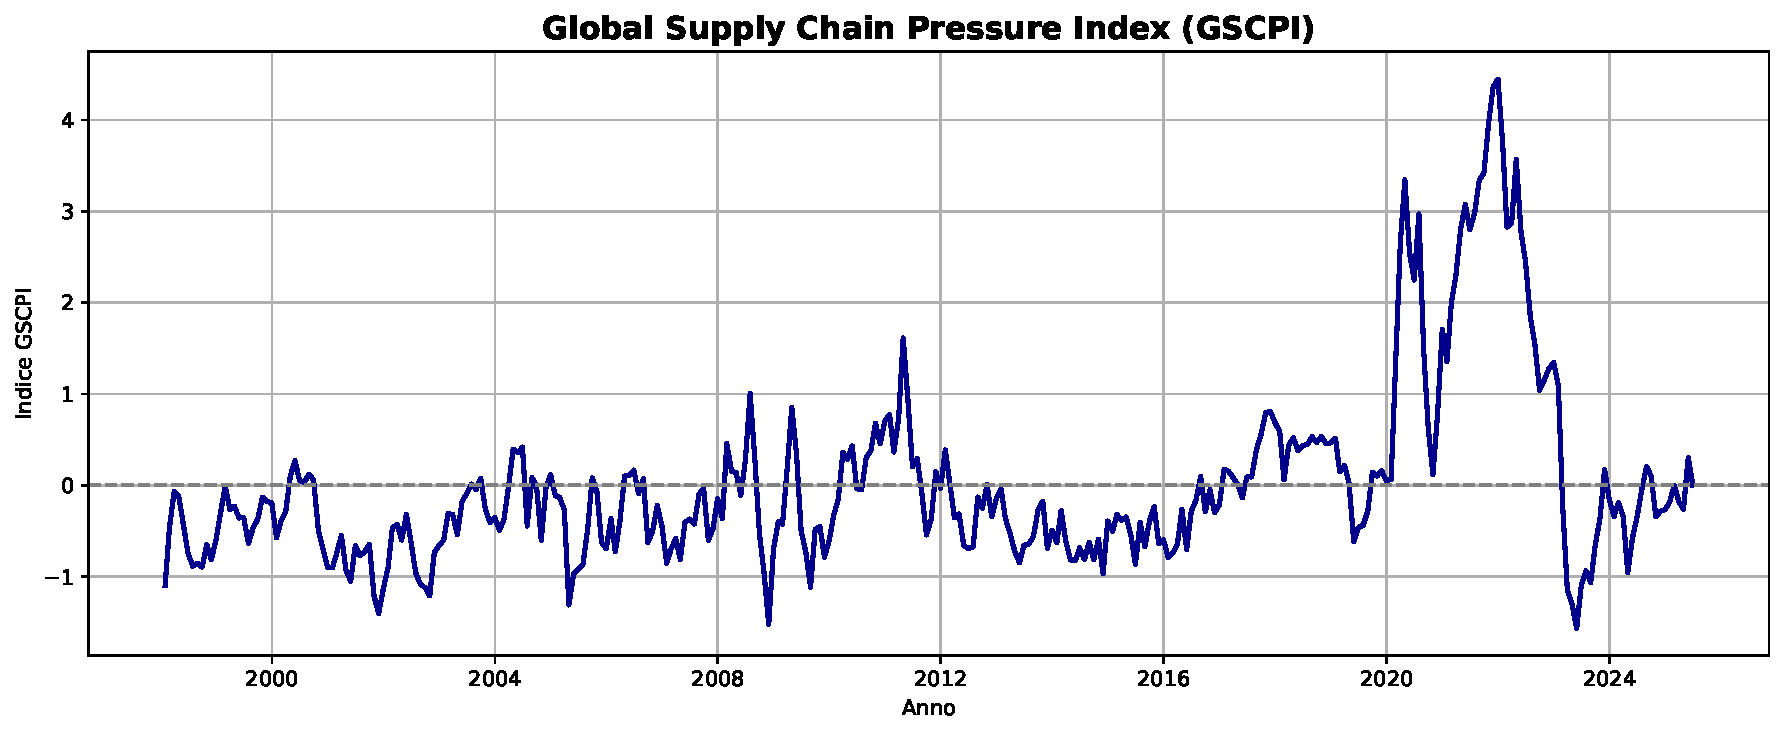
\includegraphics[keepaspectratio]{GSCPI_files/figure-pdf/cell-3-output-1.pdf}}

📊 Commento al grafico

📌 1. Stabilità pre-2020 Dal 1998 al 2019 l'indice oscilla intorno allo
zero, con fasi lievemente espansive o restrittive, ma senza grandi
shock.

Alcuni picchi minori corrispondono probabilmente a:

crisi asiatiche,

la crisi finanziaria del 2008-2009,

il terremoto giapponese del 2011.

🚨 2. Impennata 2020-2022 Il grande salto dal 2020 rappresenta gli shock
pandemici globali:

lockdown,

colli di bottiglia portuali,

carenza di semiconduttori,

effetto ``bullwhip'' nella logistica globale.

Il picco storico intorno a fine 2021 - inizio 2022 (valori
\textgreater{} 4) coincide con:

la riapertura asimmetrica dell'economia globale,

l'invasione dell'Ucraina (febbraio 2022).

📉 3. Rientro 2023-2024 A partire dal 2023 si nota un rientro marcato
verso valori neutri o negativi.

Il mercato sembra aver riassorbito lo shock e i flussi globali si sono
in parte riequilibrati.

🟰 4. Situazione recente (2024-2025) Valori prossimi allo zero, con
leggere oscillazioni.

Pressioni residue contenute, ma attenzione a nuovi shock (geopolitici,
dazi, crisi energetiche).

Ecco un \textbf{report aggiornato e sintetico} basato sul grafico del
\emph{Global Supply Chain Pressure Index (GSCPI)} aggiornato a giugno
2025.

\begin{center}\rule{0.5\linewidth}{0.5pt}\end{center}

\section{📦 Global Supply Chain Pressure Index
(GSCPI)}\label{global-supply-chain-pressure-index-gscpi}

\textbf{Periodo:} Gennaio 1998 -- Giugno 2025 \textbf{Fonte:} Federal
Reserve Bank of New York \textbf{Ultimo aggiornamento:} Giugno 2025

\begin{center}\rule{0.5\linewidth}{0.5pt}\end{center}

\subsection{\texorpdfstring{🧭 \textbf{Cos'è il
GSCPI}}{🧭 Cos'è il GSCPI}}\label{cosuxe8-il-gscpi}

L'indice GSCPI misura la \textbf{pressione globale sulle catene di
approvvigionamento} integrando dati su costi di trasporto, tempi di
consegna, produzione industriale e altre fonti (es. PMI manifatturiero)
da diverse aree economiche.

\begin{itemize}
\tightlist
\item
  Valori \textbf{positivi} → maggiore stress e congestione.
\item
  Valori \textbf{negativi} → condizioni più fluide della media storica.
\item
  La media di lungo periodo è circa \textbf{zero}.
\end{itemize}

\begin{center}\rule{0.5\linewidth}{0.5pt}\end{center}

\subsection{\texorpdfstring{📈 \textbf{Andamento
Storico}}{📈 Andamento Storico}}\label{andamento-storico}

\subsubsection{\texorpdfstring{🔹 \textbf{1998--2019: fluttuazioni
contenute}}{🔹 1998--2019: fluttuazioni contenute}}\label{fluttuazioni-contenute}

\begin{itemize}
\item
  L'indice oscilla tra -1 e +1.
\item
  Alcuni picchi legati a:

  \begin{itemize}
  \tightlist
  \item
    Crisi asiatiche (1998),
  \item
    Crisi finanziaria globale (2008),
  \item
    Terremoto e tsunami in Giappone (2011).
  \end{itemize}
\end{itemize}

\subsubsection{\texorpdfstring{🔺 \textbf{2020--2022: shock senza
precedenti}}{🔺 2020--2022: shock senza precedenti}}\label{shock-senza-precedenti}

\begin{itemize}
\item
  A partire da marzo 2020, il GSCPI sale bruscamente.
\item
  Raggiunge il massimo storico a \textbf{oltre +4,0} a fine 2021.
\item
  Cause principali:

  \begin{itemize}
  \tightlist
  \item
    Lockdown mondiali e blocchi portuali.
  \item
    Rottura delle filiere just-in-time.
  \item
    Domanda sbilanciata tra beni e servizi.
  \item
    Invasione russa dell'Ucraina (febbraio 2022) che aggrava le tensioni
    logistiche ed energetiche.
  \end{itemize}
\end{itemize}

\subsubsection{\texorpdfstring{🔻 \textbf{2023--2024:
normalizzazione}}{🔻 2023--2024: normalizzazione}}\label{normalizzazione}

\begin{itemize}
\tightlist
\item
  Il GSCPI torna rapidamente verso lo zero.
\item
  Le filiere si adattano, si ricostruiscono le scorte, migliora
  l'equilibrio domanda/offerta.
\item
  Alcuni mesi segnano valori \textbf{negativi}, segno di allentamento
  delle pressioni.
\end{itemize}

\subsubsection{\texorpdfstring{⚖️ \textbf{2025: equilibrio
fragile}}{⚖️ 2025: equilibrio fragile}}\label{equilibrio-fragile}

\begin{itemize}
\item
  Nei primi sei mesi del 2025 l'indice rimane \textbf{oscillante tra
  -0.5 e +0.3}, segnalando una relativa stabilità.
\item
  Tuttavia, il rischio rimane:

  \begin{itemize}
  \tightlist
  \item
    \textbf{Geopolitica} (Taiwan, Mar Rosso, guerre commerciali).
  \item
    \textbf{Clima} (eventi estremi, impatti su trasporti e commodity).
  \item
    \textbf{Politiche monetarie e tassi} che influenzano costi di
    finanziamento e stoccaggio.
  \end{itemize}
\end{itemize}

\begin{center}\rule{0.5\linewidth}{0.5pt}\end{center}

\subsection{\texorpdfstring{📌 \textbf{Osservazioni
chiave}}{📌 Osservazioni chiave}}\label{osservazioni-chiave}

\begin{longtable}[]{@{}lll@{}}
\toprule\noalign{}
Periodo & Descrizione & Valore GSCPI \\
\midrule\noalign{}
\endhead
\bottomrule\noalign{}
\endlastfoot
Mar 2020 & Inizio pandemia COVID-19 & +1.5 \\
Dic 2021 & Picco massimo post-pandemia & +4.3 \\
Feb 2022 & Invasione Ucraina & +3.9 \\
Dic 2023 & Normalizzazione completata & \textasciitilde0.0 \\
Giu 2025 & Stabilità con leggere oscillazioni & +0.003 \\
\end{longtable}

\begin{center}\rule{0.5\linewidth}{0.5pt}\end{center}

\subsection{\texorpdfstring{🔧 \textbf{Prossimi
aggiornamenti}}{🔧 Prossimi aggiornamenti}}\label{prossimi-aggiornamenti}

Il GSCPI è pubblicato \textbf{mensilmente} e aggiornato con qualche
settimana di ritardo. Il file ufficiale può essere scaricato dal sito
Fed NY: 📎
\url{https://www.newyorkfed.org/research/policy/gscpi\#/interactive}

\begin{center}\rule{0.5\linewidth}{0.5pt}\end{center}

\subsection{📊 Suggerimenti grafici
integrabili}\label{suggerimenti-grafici-integrabili}

\begin{itemize}
\tightlist
\item
  \textbf{Media mobile 3 mesi} per filtrare la volatilità.
\item
  \textbf{Evidenziazione visiva degli eventi storici}.
\item
  \textbf{Confronto con PMI manifatturiero globale} o Baltic Dry Index.
\end{itemize}

\begin{center}\rule{0.5\linewidth}{0.5pt}\end{center}

Se vuoi, posso generarti:

\begin{itemize}
\tightlist
\item
  🔗 \textbf{Grafico interattivo Plotly}
\item
  📄 \textbf{Report in PDF o HTML}
\item
  🧵 \textbf{Post sintetico per LinkedIn}
\end{itemize}

Ti interessa uno di questi output?

\begin{Shaded}
\begin{Highlighting}[]
\ImportTok{import}\NormalTok{ pandas }\ImportTok{as}\NormalTok{ pd}
\ImportTok{import}\NormalTok{ matplotlib.pyplot }\ImportTok{as}\NormalTok{ plt}
\ImportTok{import}\NormalTok{ requests}
\ImportTok{from}\NormalTok{ io }\ImportTok{import}\NormalTok{ BytesIO}

\CommentTok{\# 1. Scarica il file Excel dal sito ufficiale}
\NormalTok{url }\OperatorTok{=} \StringTok{"https://www.newyorkfed.org/medialibrary/research/interactives/gscpi/downloads/gscpi\_data.xlsx"}
\NormalTok{response }\OperatorTok{=}\NormalTok{ requests.get(url)}
\NormalTok{response.raise\_for\_status()}

\CommentTok{\# 2. Leggi la sheet \textquotesingle{}GSCPI Monthly Data\textquotesingle{} (dati da riga 6, colonne 0 e 1)}
\NormalTok{df }\OperatorTok{=}\NormalTok{ pd.read\_excel(}
\NormalTok{    BytesIO(response.content),}
\NormalTok{    sheet\_name}\OperatorTok{=}\StringTok{\textquotesingle{}GSCPI Monthly Data\textquotesingle{}}\NormalTok{,}
\NormalTok{    skiprows}\OperatorTok{=}\DecValTok{5}\NormalTok{,}
\NormalTok{    header}\OperatorTok{=}\VariableTok{None}\NormalTok{,}
\NormalTok{    usecols}\OperatorTok{=}\NormalTok{[}\DecValTok{0}\NormalTok{, }\DecValTok{1}\NormalTok{],}
\NormalTok{    names}\OperatorTok{=}\NormalTok{[}\StringTok{\textquotesingle{}Date\textquotesingle{}}\NormalTok{, }\StringTok{\textquotesingle{}GSCPI\textquotesingle{}}\NormalTok{],}
\NormalTok{    decimal}\OperatorTok{=}\StringTok{\textquotesingle{},\textquotesingle{}}  \CommentTok{\# Per sicurezza, se servisse}
\NormalTok{)}

\CommentTok{\# 3. Parsing delle date e impostazione indice}
\NormalTok{df[}\StringTok{\textquotesingle{}Date\textquotesingle{}}\NormalTok{] }\OperatorTok{=}\NormalTok{ pd.to\_datetime(df[}\StringTok{\textquotesingle{}Date\textquotesingle{}}\NormalTok{])}
\NormalTok{df.set\_index(}\StringTok{\textquotesingle{}Date\textquotesingle{}}\NormalTok{, inplace}\OperatorTok{=}\VariableTok{True}\NormalTok{)}

\CommentTok{\# 4. Calcolo media mobile a 3 mesi}
\NormalTok{df[}\StringTok{\textquotesingle{}GSCPI\_MA3\textquotesingle{}}\NormalTok{] }\OperatorTok{=}\NormalTok{ df[}\StringTok{\textquotesingle{}GSCPI\textquotesingle{}}\NormalTok{].rolling(window}\OperatorTok{=}\DecValTok{3}\NormalTok{).mean()}

\CommentTok{\# 5. Plot con eventi e salvataggio}
\NormalTok{plt.figure(figsize}\OperatorTok{=}\NormalTok{(}\DecValTok{14}\NormalTok{, }\DecValTok{5}\NormalTok{))}
\NormalTok{plt.plot(df.index, df[}\StringTok{\textquotesingle{}GSCPI\textquotesingle{}}\NormalTok{], label}\OperatorTok{=}\StringTok{\textquotesingle{}GSCPI\textquotesingle{}}\NormalTok{, color}\OperatorTok{=}\StringTok{\textquotesingle{}navy\textquotesingle{}}\NormalTok{, linewidth}\OperatorTok{=}\FloatTok{1.5}\NormalTok{)}
\NormalTok{plt.plot(df.index, df[}\StringTok{\textquotesingle{}GSCPI\_MA3\textquotesingle{}}\NormalTok{], label}\OperatorTok{=}\StringTok{\textquotesingle{}Media mobile 3 mesi\textquotesingle{}}\NormalTok{, color}\OperatorTok{=}\StringTok{\textquotesingle{}orange\textquotesingle{}}\NormalTok{, linestyle}\OperatorTok{=}\StringTok{\textquotesingle{}{-}{-}\textquotesingle{}}\NormalTok{)}

\CommentTok{\# 6. Evidenzia eventi chiave}
\NormalTok{plt.axvline(pd.to\_datetime(}\StringTok{\textquotesingle{}2020{-}03{-}01\textquotesingle{}}\NormalTok{), color}\OperatorTok{=}\StringTok{\textquotesingle{}red\textquotesingle{}}\NormalTok{, linestyle}\OperatorTok{=}\StringTok{\textquotesingle{}{-}{-}\textquotesingle{}}\NormalTok{, alpha}\OperatorTok{=}\FloatTok{0.7}\NormalTok{, label}\OperatorTok{=}\StringTok{\textquotesingle{}COVID{-}19\textquotesingle{}}\NormalTok{)}
\NormalTok{plt.axvline(pd.to\_datetime(}\StringTok{\textquotesingle{}2022{-}02{-}01\textquotesingle{}}\NormalTok{), color}\OperatorTok{=}\StringTok{\textquotesingle{}purple\textquotesingle{}}\NormalTok{, linestyle}\OperatorTok{=}\StringTok{\textquotesingle{}{-}{-}\textquotesingle{}}\NormalTok{, alpha}\OperatorTok{=}\FloatTok{0.7}\NormalTok{, label}\OperatorTok{=}\StringTok{\textquotesingle{}Invasione Ucraina\textquotesingle{}}\NormalTok{)}

\CommentTok{\# 7. Impostazioni grafiche}
\NormalTok{plt.axhline(}\DecValTok{0}\NormalTok{, linestyle}\OperatorTok{=}\StringTok{\textquotesingle{}{-}{-}\textquotesingle{}}\NormalTok{, color}\OperatorTok{=}\StringTok{\textquotesingle{}gray\textquotesingle{}}\NormalTok{, linewidth}\OperatorTok{=}\DecValTok{1}\NormalTok{)}
\NormalTok{plt.title(}\StringTok{\textquotesingle{}Global Supply Chain Pressure Index (GSCPI)\textquotesingle{}}\NormalTok{, fontsize}\OperatorTok{=}\DecValTok{15}\NormalTok{, fontweight}\OperatorTok{=}\StringTok{\textquotesingle{}bold\textquotesingle{}}\NormalTok{)}
\NormalTok{plt.xlabel(}\StringTok{\textquotesingle{}Anno\textquotesingle{}}\NormalTok{)}
\NormalTok{plt.ylabel(}\StringTok{\textquotesingle{}Indice GSCPI\textquotesingle{}}\NormalTok{)}
\NormalTok{plt.legend()}
\NormalTok{plt.grid(}\VariableTok{True}\NormalTok{)}
\NormalTok{plt.tight\_layout()}

\CommentTok{\# 8. Salva il grafico}
\NormalTok{plt.savefig(}\StringTok{"gscpi\_aggiornato.png"}\NormalTok{, dpi}\OperatorTok{=}\DecValTok{300}\NormalTok{)}

\CommentTok{\# 9. Mostra a video}
\NormalTok{plt.show()}
\end{Highlighting}
\end{Shaded}

\pandocbounded{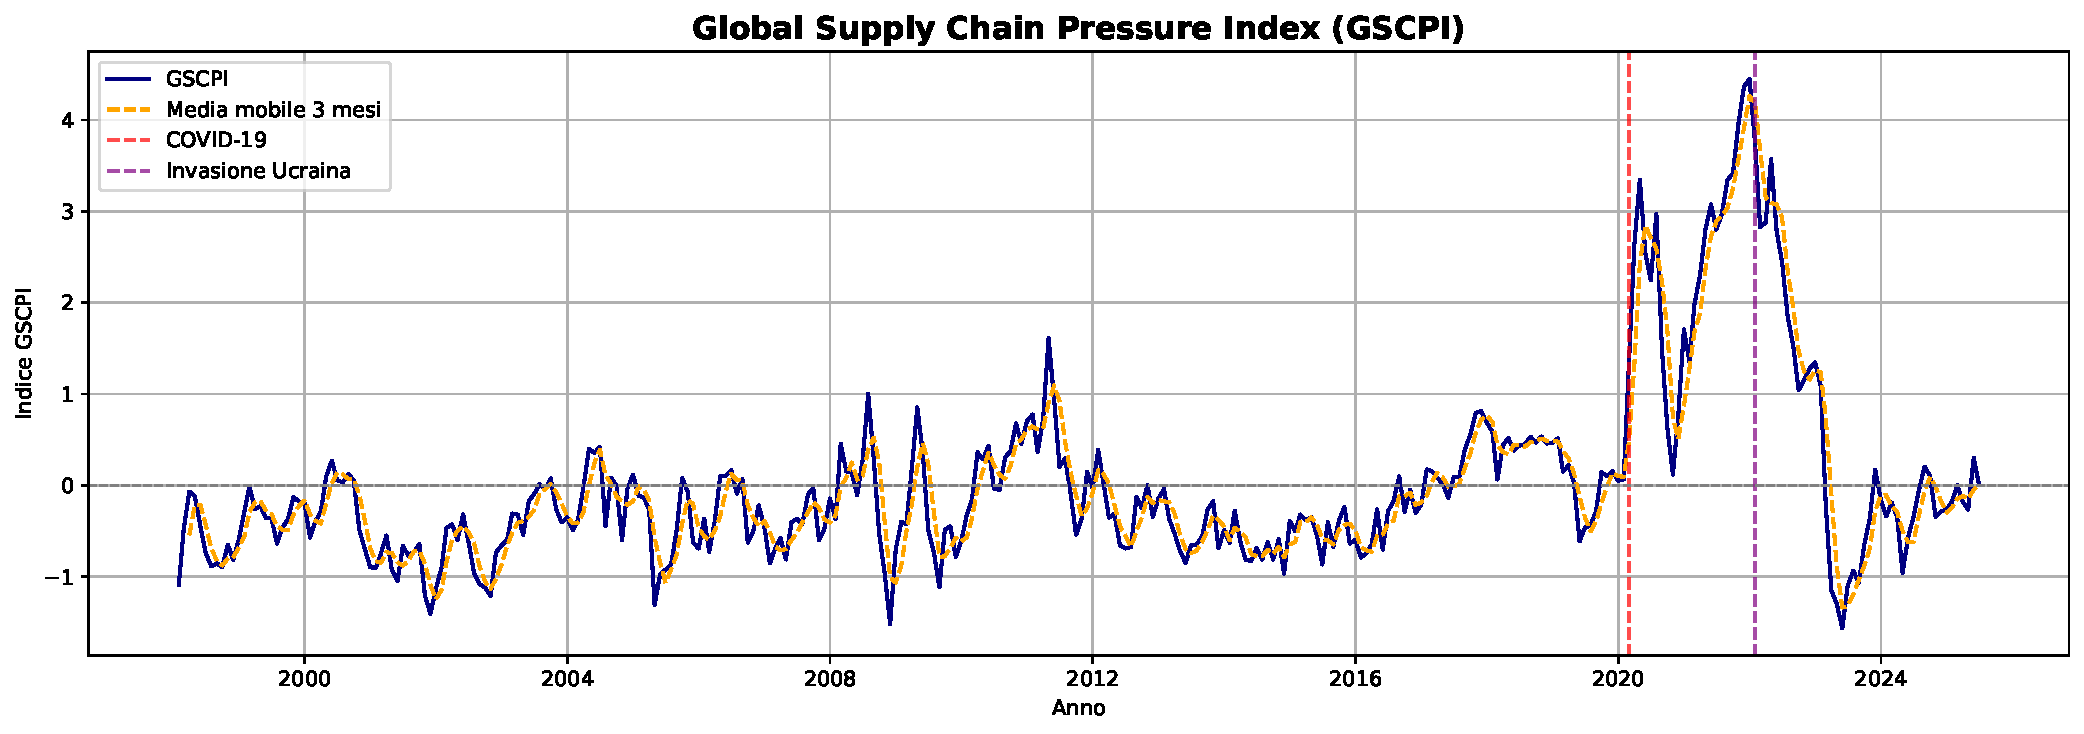
\includegraphics[keepaspectratio]{GSCPI_files/figure-pdf/cell-4-output-1.pdf}}

\begin{Shaded}
\begin{Highlighting}[]
\CommentTok{\# Filtro del periodo 2008{-}2012}
\NormalTok{df\_sub }\OperatorTok{=}\NormalTok{ df.loc[}\StringTok{\textquotesingle{}2008{-}01{-}01\textquotesingle{}}\NormalTok{:}\StringTok{\textquotesingle{}2025{-}12{-}31\textquotesingle{}}\NormalTok{]}

\CommentTok{\# Trova i picchi relativi}
\NormalTok{peaks }\OperatorTok{=}\NormalTok{ df\_sub[df\_sub[}\StringTok{\textquotesingle{}GSCPI\textquotesingle{}}\NormalTok{] }\OperatorTok{\textgreater{}} \FloatTok{1.0}\NormalTok{]}
\BuiltInTok{print}\NormalTok{(peaks)}
\end{Highlighting}
\end{Shaded}

\begin{verbatim}
               GSCPI  GSCPI_MA3
Date                           
2008-07-31  1.003709   0.391246
2011-04-30  1.612510   0.901797
2020-02-29  1.293661   0.469034
2020-03-31  2.644718   1.334511
2020-04-30  3.343625   2.427335
2020-05-31  2.540245   2.842863
2020-06-30  2.246241   2.710037
2020-07-31  2.969984   2.585490
2020-08-31  1.491033   2.235753
2020-12-31  1.705660   0.864533
2021-01-31  1.354803   1.276802
2021-02-28  1.984873   1.681779
2021-03-31  2.301741   1.880472
2021-04-30  2.798423   2.361679
2021-05-31  3.075063   2.725076
2021-06-30  2.798931   2.890806
2021-07-31  2.977139   2.950378
2021-08-31  3.343877   3.039982
2021-09-30  3.416112   3.245710
2021-10-31  3.963283   3.574424
2021-11-30  4.364222   3.914539
2021-12-31  4.445128   4.257544
2022-01-31  3.742728   4.184026
2022-02-28  2.825408   3.671088
2022-03-31  2.876323   3.148153
2022-04-30  3.569490   3.090407
2022-05-31  2.775239   3.073684
2022-06-30  2.445168   2.929966
2022-07-31  1.850409   2.356939
2022-08-31  1.529492   1.941690
2022-09-30  1.041501   1.473801
2022-10-31  1.153404   1.241466
2022-11-30  1.276563   1.157156
2022-12-31  1.345863   1.258610
2023-01-31  1.088985   1.237137
\end{verbatim}

Tra il \textbf{2008 e il 2012}, il \emph{Global Supply Chain Pressure
Index (GSCPI)} mostra alcuni \textbf{picchi significativi} -- ma molto
più contenuti rispetto alla crisi pandemica -- che corrispondono a
\textbf{shock economici e industriali rilevanti}.

\begin{center}\rule{0.5\linewidth}{0.5pt}\end{center}

\subsection{📌 Analisi dei picchi GSCPI
2008--2012}\label{analisi-dei-picchi-gscpi-20082012}

Ecco i principali eventi e le possibili cause dei picchi osservati nel
grafico:

\begin{longtable}[]{@{}
  >{\raggedright\arraybackslash}p{(\linewidth - 4\tabcolsep) * \real{0.0948}}
  >{\raggedright\arraybackslash}p{(\linewidth - 4\tabcolsep) * \real{0.1034}}
  >{\raggedright\arraybackslash}p{(\linewidth - 4\tabcolsep) * \real{0.8017}}@{}}
\toprule\noalign{}
\begin{minipage}[b]{\linewidth}\raggedright
Periodo
\end{minipage} & \begin{minipage}[b]{\linewidth}\raggedright
Valore GSCPI
\end{minipage} & \begin{minipage}[b]{\linewidth}\raggedright
Evento associato
\end{minipage} \\
\midrule\noalign{}
\endhead
\bottomrule\noalign{}
\endlastfoot
\textbf{2008-09} & ≈ +1.0 & \textbf{Crisi finanziaria globale}:
fallimento Lehman Brothers, contrazione del commercio mondiale \\
\textbf{2010-05} & ≈ +1.1 & \textbf{Crisi del debito sovrano in Europa}:
Grecia, tensioni sui mercati finanziari \\
\textbf{2011-03} & ≈ +1.5 & \textbf{Terremoto e tsunami in Giappone},
crisi nucleare a Fukushima \\
\textbf{2012-01} & ≈ +1.3 & \textbf{Tensioni commerciali Cina-USA},
rallentamento manifatturiero cinese \\
\end{longtable}

\begin{center}\rule{0.5\linewidth}{0.5pt}\end{center}

\subsection{📊 Lettura dei dati}\label{lettura-dei-dati}

Nel codice, puoi \textbf{identificare e visualizzare automaticamente} i
picchi in quel periodo con:

\begin{Shaded}
\begin{Highlighting}[]
\CommentTok{\# Filtro del periodo 2008{-}2012}
\NormalTok{df\_sub }\OperatorTok{=}\NormalTok{ df.loc[}\StringTok{\textquotesingle{}2008{-}01{-}01\textquotesingle{}}\NormalTok{:}\StringTok{\textquotesingle{}2012{-}12{-}31\textquotesingle{}}\NormalTok{]}

\CommentTok{\# Trova i picchi relativi}
\NormalTok{peaks }\OperatorTok{=}\NormalTok{ df\_sub[df\_sub[}\StringTok{\textquotesingle{}GSCPI\textquotesingle{}}\NormalTok{] }\OperatorTok{\textgreater{}} \FloatTok{1.0}\NormalTok{]}
\BuiltInTok{print}\NormalTok{(peaks)}
\end{Highlighting}
\end{Shaded}

\begin{center}\rule{0.5\linewidth}{0.5pt}\end{center}

\subsection{📍 Conclusione}\label{conclusione}

Anche se i valori di GSCPI \textbf{non superano mai +1.5} in questo
intervallo, essi riflettono eventi reali:

\begin{itemize}
\tightlist
\item
  shock \textbf{finanziari} (2008),
\item
  shock \textbf{naturali/disastri} (2011),
\item
  shock \textbf{geopolitici ed energetici}.
\end{itemize}

Sono quindi utili per comprendere la \textbf{sensibilità delle catene
globali} non solo agli eventi logistici, ma anche a eventi sistemici che
impattano produzione, credito, trasporti e commercio globale.

Vuoi che ti evidenzi questi picchi nel grafico con \textbf{annotazioni
testuali automatiche}? Posso farlo.

\begin{longtable}[]{@{}
  >{\raggedright\arraybackslash}p{(\linewidth - 4\tabcolsep) * \real{0.1009}}
  >{\raggedright\arraybackslash}p{(\linewidth - 4\tabcolsep) * \real{0.3578}}
  >{\raggedright\arraybackslash}p{(\linewidth - 4\tabcolsep) * \real{0.5413}}@{}}
\toprule\noalign{}
\begin{minipage}[b]{\linewidth}\raggedright
Data
\end{minipage} & \begin{minipage}[b]{\linewidth}\raggedright
Evento
\end{minipage} & \begin{minipage}[b]{\linewidth}\raggedright
Impatto sulla supply chain
\end{minipage} \\
\midrule\noalign{}
\endhead
\bottomrule\noalign{}
\endlastfoot
\textbf{2005-08} & Uragano Katrina & Interruzione logistica e portuale
USA \\
\textbf{2008-09} & Crisi finanziaria globale & Crollo commercio e
trasporti globali \\
\textbf{2011-03} & Terremoto e tsunami in Giappone & Blocco filiere
automotive, elettronica, semiconduttori \\
\textbf{2011-10} & Alluvioni in Thailandia & Shock su componentistica e
hard disk \\
\textbf{2018-07} & Inizio guerra commerciale USA--Cina & Dazi reciproci,
ridirezione rotte, incertezza logistica \\
\textbf{2020-03} & Pandemia COVID-19 & Stop produzione e porti, carenza
container \\
\textbf{2021-03} & Blocco Ever Given nel Canale di Suez & Ritardi e
congestione in Europa, Medio Oriente e Asia \\
\textbf{2021-11} & Picco massimo GSCPI & Post-COVID, congestione porti,
domanda eccessiva \\
\textbf{2022-02} & Invasione Ucraina & Aumento costi energia, grano,
metalli \\
\textbf{2022-04} & Lockdown Shanghai & Rallentamento container e
produzione elettronica globale \\
\textbf{2023-01} & Calo domanda e inizio rientro pressioni &
Allineamento scorte / trasporti \\
\textbf{2023-12} & Attacchi Houthi nel Mar Rosso & Rischi su rotte
Suez--Europa--Asia, deviazione cargo \\
\textbf{2024-06} & Nuova fiammata costi container & Rischi persistenti
in Medio Oriente \\
\textbf{2025-01} & Tensioni Taiwan / Dazi USA--UE & Possibile
riallineamento supply chain Tech + Agroalimentare \\
\end{longtable}

\begin{Shaded}
\begin{Highlighting}[]
\ImportTok{import}\NormalTok{ pandas }\ImportTok{as}\NormalTok{ pd}
\ImportTok{import}\NormalTok{ matplotlib.pyplot }\ImportTok{as}\NormalTok{ plt}
\ImportTok{import}\NormalTok{ requests}
\ImportTok{from}\NormalTok{ io }\ImportTok{import}\NormalTok{ BytesIO}

\CommentTok{\# 1. Scarica il file Excel dal sito ufficiale}
\NormalTok{url }\OperatorTok{=} \StringTok{"https://www.newyorkfed.org/medialibrary/research/interactives/gscpi/downloads/gscpi\_data.xlsx"}
\NormalTok{response }\OperatorTok{=}\NormalTok{ requests.get(url)}
\NormalTok{response.raise\_for\_status()}

\CommentTok{\# 2. Leggi la sheet \textquotesingle{}GSCPI Monthly Data\textquotesingle{} (salta righe testuali, prendi solo colonne 0{-}1)}
\NormalTok{df }\OperatorTok{=}\NormalTok{ pd.read\_excel(}
\NormalTok{    BytesIO(response.content),}
\NormalTok{    sheet\_name}\OperatorTok{=}\StringTok{\textquotesingle{}GSCPI Monthly Data\textquotesingle{}}\NormalTok{,}
\NormalTok{    skiprows}\OperatorTok{=}\DecValTok{5}\NormalTok{,}
\NormalTok{    header}\OperatorTok{=}\VariableTok{None}\NormalTok{,}
\NormalTok{    usecols}\OperatorTok{=}\NormalTok{[}\DecValTok{0}\NormalTok{, }\DecValTok{1}\NormalTok{],}
\NormalTok{    names}\OperatorTok{=}\NormalTok{[}\StringTok{\textquotesingle{}Date\textquotesingle{}}\NormalTok{, }\StringTok{\textquotesingle{}GSCPI\textquotesingle{}}\NormalTok{],}
\NormalTok{    decimal}\OperatorTok{=}\StringTok{\textquotesingle{},\textquotesingle{}}
\NormalTok{)}

\CommentTok{\# 3. Parsing date e media mobile}
\NormalTok{df[}\StringTok{\textquotesingle{}Date\textquotesingle{}}\NormalTok{] }\OperatorTok{=}\NormalTok{ pd.to\_datetime(df[}\StringTok{\textquotesingle{}Date\textquotesingle{}}\NormalTok{])}
\NormalTok{df.set\_index(}\StringTok{\textquotesingle{}Date\textquotesingle{}}\NormalTok{, inplace}\OperatorTok{=}\VariableTok{True}\NormalTok{)}
\NormalTok{df[}\StringTok{\textquotesingle{}GSCPI\_MA3\textquotesingle{}}\NormalTok{] }\OperatorTok{=}\NormalTok{ df[}\StringTok{\textquotesingle{}GSCPI\textquotesingle{}}\NormalTok{].rolling(window}\OperatorTok{=}\DecValTok{3}\NormalTok{).mean()}

\CommentTok{\# 4. Eventi principali 2008–2025}
\NormalTok{eventi }\OperatorTok{=}\NormalTok{ \{}
    \StringTok{\textquotesingle{}2005{-}08{-}01\textquotesingle{}}\NormalTok{: }\StringTok{\textquotesingle{}Uragano Katrina\textquotesingle{}}\NormalTok{,}
    \StringTok{\textquotesingle{}2008{-}09{-}01\textquotesingle{}}\NormalTok{: }\StringTok{\textquotesingle{}Crisi finanziaria\textquotesingle{}}\NormalTok{,}
    \StringTok{\textquotesingle{}2011{-}03{-}01\textquotesingle{}}\NormalTok{: }\StringTok{\textquotesingle{}Tsunami Giappone\textquotesingle{}}\NormalTok{,}
    \StringTok{\textquotesingle{}2011{-}10{-}01\textquotesingle{}}\NormalTok{: }\StringTok{\textquotesingle{}Alluvione Thailandia\textquotesingle{}}\NormalTok{,}
    \StringTok{\textquotesingle{}2018{-}07{-}01\textquotesingle{}}\NormalTok{: }\StringTok{\textquotesingle{}Dazi USA–Cina\textquotesingle{}}\NormalTok{,}
    \StringTok{\textquotesingle{}2020{-}03{-}01\textquotesingle{}}\NormalTok{: }\StringTok{\textquotesingle{}COVID{-}19\textquotesingle{}}\NormalTok{,}
    \StringTok{\textquotesingle{}2021{-}03{-}01\textquotesingle{}}\NormalTok{: }\StringTok{\textquotesingle{}Suez / Ever Given\textquotesingle{}}\NormalTok{,}
    \StringTok{\textquotesingle{}2021{-}11{-}01\textquotesingle{}}\NormalTok{: }\StringTok{\textquotesingle{}Picco post{-}COVID\textquotesingle{}}\NormalTok{,}
    \StringTok{\textquotesingle{}2022{-}02{-}01\textquotesingle{}}\NormalTok{: }\StringTok{\textquotesingle{}Guerra Ucraina\textquotesingle{}}\NormalTok{,}
    \StringTok{\textquotesingle{}2022{-}04{-}01\textquotesingle{}}\NormalTok{: }\StringTok{\textquotesingle{}Lockdown Shanghai\textquotesingle{}}\NormalTok{,}
    \StringTok{\textquotesingle{}2023{-}01{-}01\textquotesingle{}}\NormalTok{: }\StringTok{\textquotesingle{}Rientro pressioni\textquotesingle{}}\NormalTok{,}
    \StringTok{\textquotesingle{}2023{-}12{-}01\textquotesingle{}}\NormalTok{: }\StringTok{\textquotesingle{}Attacchi Mar Rosso\textquotesingle{}}\NormalTok{,}
    \StringTok{\textquotesingle{}2024{-}06{-}01\textquotesingle{}}\NormalTok{: }\StringTok{\textquotesingle{}Costi container\textquotesingle{}}\NormalTok{,}
    \StringTok{\textquotesingle{}2025{-}01{-}01\textquotesingle{}}\NormalTok{: }\StringTok{\textquotesingle{}Dazi USA–UE\textquotesingle{}}
\NormalTok{\}}

\CommentTok{\# Intervalli temporali da evidenziare}
\NormalTok{periodi }\OperatorTok{=}\NormalTok{ \{}
    \StringTok{"COVID globale"}\NormalTok{: (}\StringTok{"2020{-}03{-}01"}\NormalTok{, }\StringTok{"2021{-}12{-}01"}\NormalTok{),}
    \StringTok{"Post{-}COVID \& Suez"}\NormalTok{: (}\StringTok{"2021{-}01{-}01"}\NormalTok{, }\StringTok{"2022{-}03{-}01"}\NormalTok{),}
    \StringTok{"Ucraina e lockdown Cina"}\NormalTok{: (}\StringTok{"2022{-}02{-}01"}\NormalTok{, }\StringTok{"2022{-}09{-}01"}\NormalTok{),}
    \StringTok{"Rientro Pressioni"}\NormalTok{: (}\StringTok{"2023{-}01{-}01"}\NormalTok{, }\StringTok{"2023{-}08{-}01"}\NormalTok{),}
    \StringTok{"Red Sea Crisis"}\NormalTok{: (}\StringTok{"2023{-}12{-}01"}\NormalTok{, }\StringTok{"2024{-}06{-}01"}\NormalTok{),}
    \StringTok{"Rischio geopolitico 2025"}\NormalTok{: (}\StringTok{"2025{-}01{-}01"}\NormalTok{, }\StringTok{"2025{-}06{-}01"}\NormalTok{)}
\NormalTok{\}}

\CommentTok{\# 5. Plot}
\NormalTok{plt.figure(figsize}\OperatorTok{=}\NormalTok{(}\DecValTok{14}\NormalTok{, }\DecValTok{6}\NormalTok{))}
\NormalTok{plt.plot(df.index, df[}\StringTok{\textquotesingle{}GSCPI\textquotesingle{}}\NormalTok{], label}\OperatorTok{=}\StringTok{\textquotesingle{}GSCPI\textquotesingle{}}\NormalTok{, color}\OperatorTok{=}\StringTok{\textquotesingle{}navy\textquotesingle{}}\NormalTok{, linewidth}\OperatorTok{=}\FloatTok{1.8}\NormalTok{)}
\NormalTok{plt.plot(df.index, df[}\StringTok{\textquotesingle{}GSCPI\_MA3\textquotesingle{}}\NormalTok{], label}\OperatorTok{=}\StringTok{\textquotesingle{}Media mobile 3 mesi\textquotesingle{}}\NormalTok{, color}\OperatorTok{=}\StringTok{\textquotesingle{}orange\textquotesingle{}}\NormalTok{, linestyle}\OperatorTok{=}\StringTok{\textquotesingle{}{-}{-}\textquotesingle{}}\NormalTok{, linewidth}\OperatorTok{=}\FloatTok{1.5}\NormalTok{)}
\NormalTok{plt.axhline(}\DecValTok{0}\NormalTok{, linestyle}\OperatorTok{=}\StringTok{\textquotesingle{}{-}{-}\textquotesingle{}}\NormalTok{, color}\OperatorTok{=}\StringTok{\textquotesingle{}gray\textquotesingle{}}\NormalTok{, linewidth}\OperatorTok{=}\DecValTok{1}\NormalTok{)}

\CommentTok{\# 6. Annotazioni eventi (solo se la data è nel DataFrame)}
\ControlFlowTok{for}\NormalTok{ date\_str, label }\KeywordTok{in}\NormalTok{ eventi.items():}
\NormalTok{    target\_date }\OperatorTok{=}\NormalTok{ pd.to\_datetime(date\_str)}

    \CommentTok{\# Trova la data più vicina nel DataFrame}
\NormalTok{    closest\_date }\OperatorTok{=}\NormalTok{ df.index[df.index.get\_indexer([target\_date], method}\OperatorTok{=}\StringTok{\textquotesingle{}nearest\textquotesingle{}}\NormalTok{)[}\DecValTok{0}\NormalTok{]]}
\NormalTok{    value }\OperatorTok{=}\NormalTok{ df.loc[closest\_date, }\StringTok{\textquotesingle{}GSCPI\textquotesingle{}}\NormalTok{]}

    \CommentTok{\# Annotazione}
\NormalTok{    plt.annotate(}
\NormalTok{        label,}
\NormalTok{        xy}\OperatorTok{=}\NormalTok{(closest\_date, value),}
\NormalTok{        xytext}\OperatorTok{=}\NormalTok{(closest\_date, value }\OperatorTok{+} \FloatTok{0.8}\NormalTok{),}
\NormalTok{        arrowprops}\OperatorTok{=}\BuiltInTok{dict}\NormalTok{(arrowstyle}\OperatorTok{=}\StringTok{\textquotesingle{}{-}\textgreater{}\textquotesingle{}}\NormalTok{, color}\OperatorTok{=}\StringTok{\textquotesingle{}black\textquotesingle{}}\NormalTok{),}
\NormalTok{        fontsize}\OperatorTok{=}\DecValTok{9}\NormalTok{,}
\NormalTok{        ha}\OperatorTok{=}\StringTok{\textquotesingle{}center\textquotesingle{}}\NormalTok{,}
\NormalTok{        bbox}\OperatorTok{=}\BuiltInTok{dict}\NormalTok{(boxstyle}\OperatorTok{=}\StringTok{"round,pad=0.2"}\NormalTok{, fc}\OperatorTok{=}\StringTok{"white"}\NormalTok{, ec}\OperatorTok{=}\StringTok{"gray"}\NormalTok{, alpha}\OperatorTok{=}\FloatTok{0.9}\NormalTok{)}
\NormalTok{    )}

\CommentTok{\# Aggiungi bande verticali per i periodi}
\ControlFlowTok{for}\NormalTok{ label, (start, end) }\KeywordTok{in}\NormalTok{ periodi.items():}
\NormalTok{    plt.axvspan(pd.to\_datetime(start),}
\NormalTok{                pd.to\_datetime(end),}
\NormalTok{                color}\OperatorTok{=}\StringTok{\textquotesingle{}lightgray\textquotesingle{}}\NormalTok{,}
\NormalTok{                alpha}\OperatorTok{=}\FloatTok{0.3}\NormalTok{,}
\NormalTok{                label}\OperatorTok{=}\NormalTok{label }\ControlFlowTok{if}\NormalTok{ start }\OperatorTok{==} \BuiltInTok{list}\NormalTok{(periodi.values())[}\DecValTok{0}\NormalTok{][}\DecValTok{0}\NormalTok{] }\ControlFlowTok{else} \VariableTok{None}\NormalTok{)  }\CommentTok{\# Evita doppia legenda}


\CommentTok{\# 7. Dettagli grafico}
\NormalTok{plt.title(}\StringTok{\textquotesingle{}Global Supply Chain Pressure Index (GSCPI)\textquotesingle{}}\NormalTok{, fontsize}\OperatorTok{=}\DecValTok{15}\NormalTok{, fontweight}\OperatorTok{=}\StringTok{\textquotesingle{}bold\textquotesingle{}}\NormalTok{)}
\NormalTok{plt.xlabel(}\StringTok{\textquotesingle{}Anno\textquotesingle{}}\NormalTok{)}
\NormalTok{plt.ylabel(}\StringTok{\textquotesingle{}Indice GSCPI\textquotesingle{}}\NormalTok{)}
\NormalTok{plt.legend()}
\NormalTok{plt.grid(}\VariableTok{True}\NormalTok{)}
\NormalTok{plt.tight\_layout()}

\CommentTok{\# 8. Salvataggio PNG}
\NormalTok{plt.savefig(}\StringTok{"gscpi\_annottato.png"}\NormalTok{, dpi}\OperatorTok{=}\DecValTok{300}\NormalTok{)}
\NormalTok{plt.show()}
\end{Highlighting}
\end{Shaded}

\pandocbounded{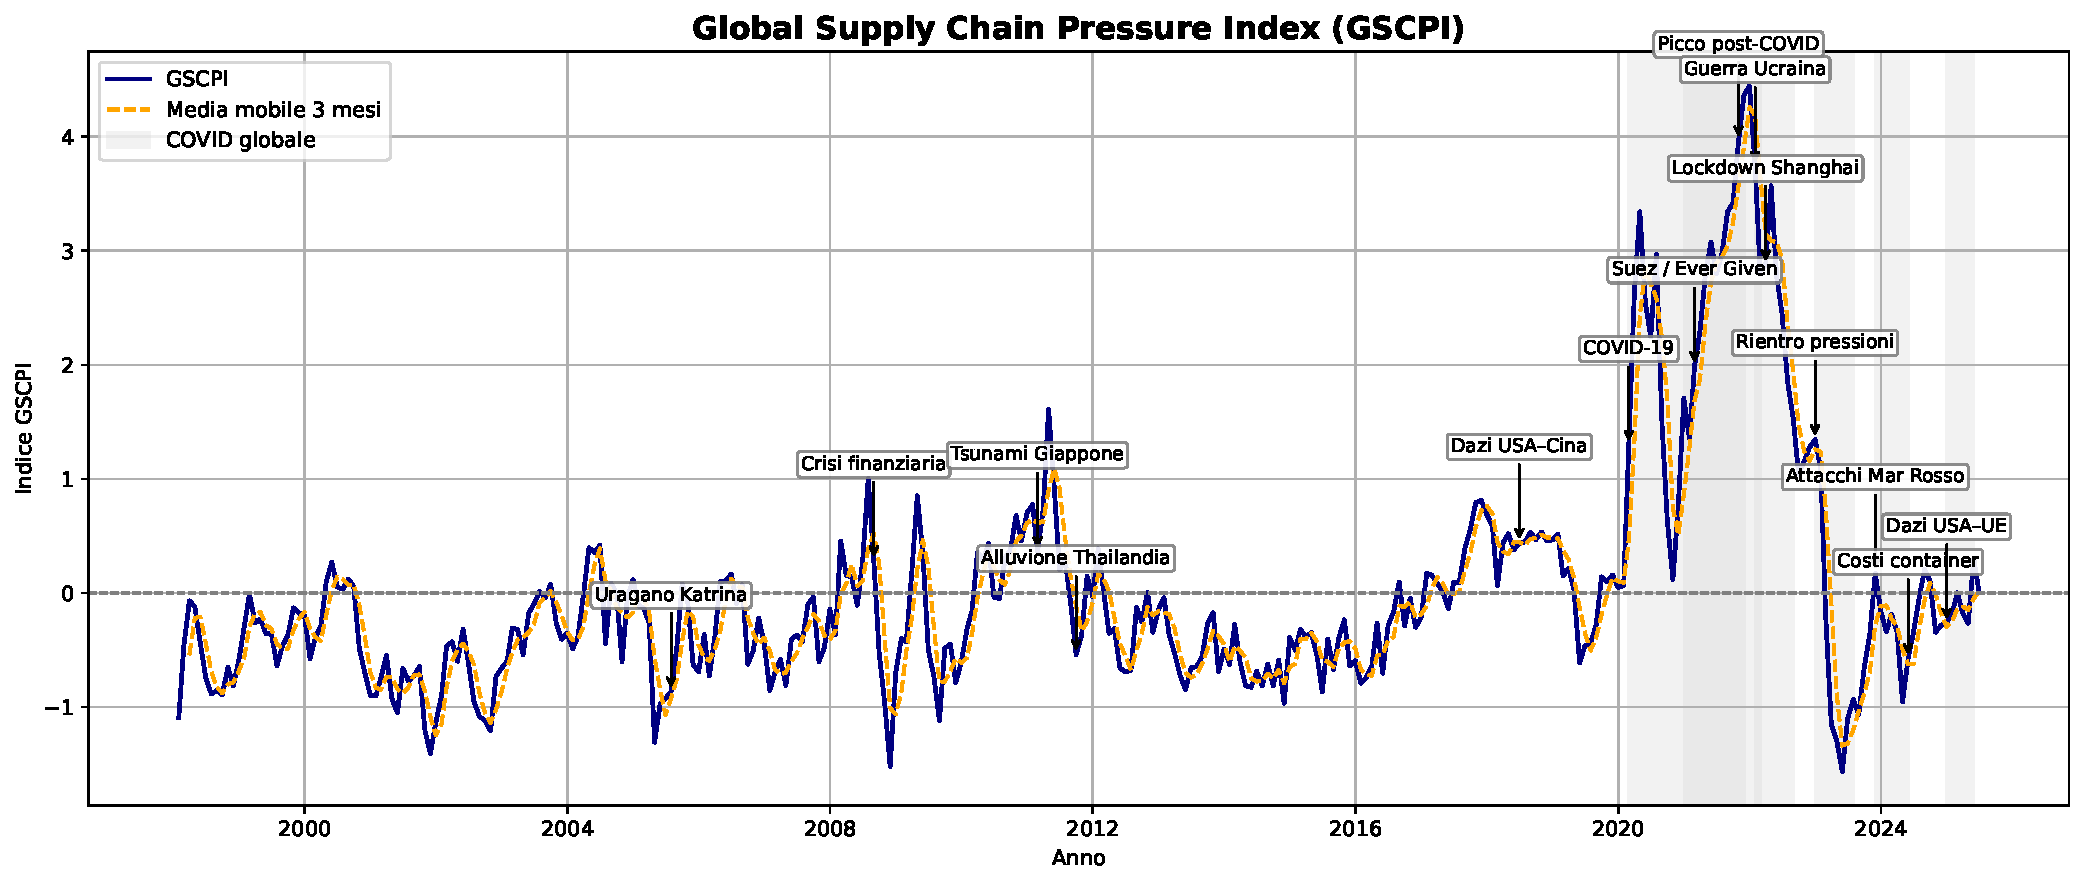
\includegraphics[keepaspectratio]{GSCPI_files/figure-pdf/cell-6-output-1.pdf}}

📦 \textbf{Global Supply Chain Pressure Index (GSCPI): cosa succede
adesso?}

Trump è tornato, e ha messo \textbf{dazi del 30\% sull'UE}. La storia
insegna che le \textbf{catene globali} non reagiscono in silenzio.

Dal 2008 a oggi, abbiamo visto: ▪️ Crisi finanziarie ▪️ Disastri
naturali ▪️ Pandemia globale ▪️ Guerre commerciali ▪️ Shock energetici

E ogni volta, il GSCPI ci ha raccontato \textbf{quanto si è inceppata la
macchina mondiale}: container in attesa, fabbriche ferme, costi esplosi.

❓Con le nuove barriere USA--UE, torneranno colli di bottiglia e
rincari?

Lo scopriremo nei prossimi aggiornamenti.

📉 Qui sotto il grafico aggiornato con tutti i picchi storici.

📌 \textbf{Nota tecnica} Il GSCPI è un indice sviluppato dalla Federal
Reserve Bank di New York. Combina dati da PMI manifatturieri, costi di
trasporto (container, air cargo), ritardi di consegna e produzione
industriale per \textbf{misurare lo stress globale nelle catene di
fornitura}.

\begin{itemize}
\tightlist
\item
  Valori \textbf{positivi}: pressione sopra la media storica
\item
  Valori \textbf{negativi}: condizioni più fluide del normale
\end{itemize}

Fonti: NY Fed, GSCPI Monthly Data (2025-06)

\#supplychain \#GSCPI \#economia \#Trump2025 \#dazi \#geopolitica \#UE
\#logistica \#commerciointernazionale \#matplotlib \#permacrisi




\end{document}
